\chapter{Experiments}

The original implementation provided with the research paper implements SSD in the \textit{Caffe} \footnote{\url{http://caffe.berkeleyvision.org/}} deep learning framework. We decided against performing our experiments in Caffe and decided to implement our version in newer \textit{PyTorch} \footnote{\url{https://pytorch.org/}} framework. 


\section{Xception}

\begin{figure}
    \centering
    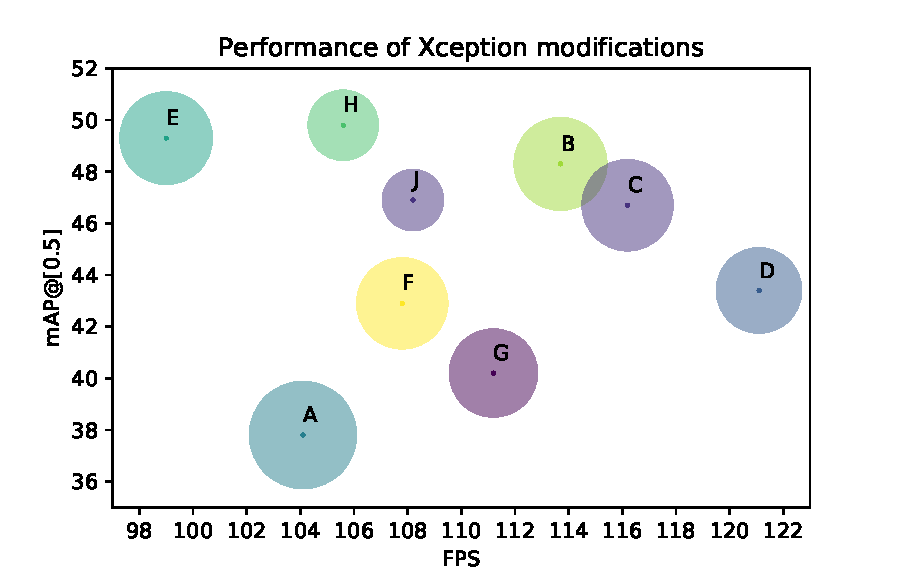
\includegraphics[width=\textwidth]{img/fps_map_x}
    \caption[Performance of multiple Xception modification on Surveillance dataset]{Performance of multiple Xception modification on Surveillance dataset. Circle diameters demonstrate relative difference of network parameter counts.} 
    \label{fig:xception_perf}
\end{figure}

\section{Precision}

\begin{figure}
    \centering
    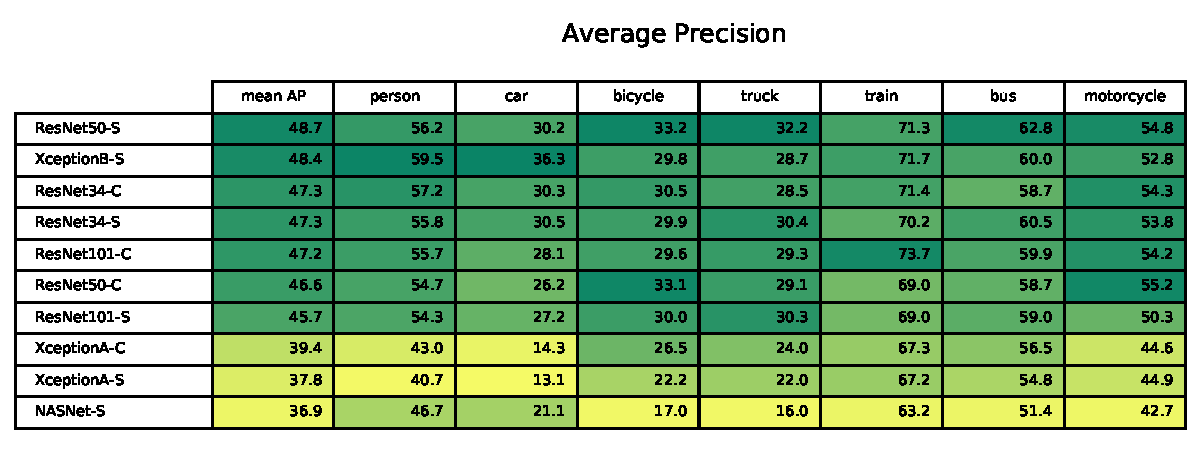
\includegraphics[width=\textwidth]{img/ap}
    \caption[Average precision of all tested networks on Surveillance dataset]{Average precision of all tested networks on Surveillance dataset. \textit{COCO} indicates that the network was trained on COCO dataset.} 
    \label{fig:ap}
\end{figure}

\section{Inference speed}
The absolute values of the inference speed measurement have no information value without the knowledge of the environment in which they have been taken. In this section, we provide the details of both software and hardware environments used for measurements.

The testing was done by timing the total time to process 10 000 images and then simply calculating the \textit{fps} value. We do not consider scaling and cropping the images to be the part of the network and therefore we had no need to include this process in the measurement, the set of [300\x300] pixel images was pre-loaded into memory. On the other hand, the non-maximum suppression is critical part of the algorithm and is included. 

\paragraph{Hardware} All our testing was done on the following hardware:
\begin{itemize}
    \item AMD EPYC 7401P CPU @ 2GHz \x 24
    \item NVIDIA GeForce GTX 1080 Ti
    \item 128GB DDR4 RAM
\end{itemize}

\section{ssdtc?}